\chapter{Background}
\label{cha:bg}

In this section, we will introduce the main concepts and technologies on which video streaming, and therefore our work, is based. We will start with video compression concepts, going through important concepts such as \textit{Group of Pictures} (GOP), also presenting some popular video codec formats. We will then delve into video container formats, introducing MPEG-2 Transport Stream, MP4 and Fragmented MP4. We will also present how adaptive bitrate streaming works and the main technologies, such as Apple HLS and MPEG-DASH, go through the evolution of HTTP versions (HTTP/3 in particular), and finally briefly introduce the main network emulation tools.

\section{Video compression concepts}
\label{sec:bg/compression}

Video is known to be one of the heaviest types of content to be stored and transmitted. Since treating uncompressed video is unfeasible, video compression or video coding formats have been developed and standardized over the years, with multiple implementations (\textbf{codecs}) being released. The objective of video codecs is to limit the output data rate, measured in bits per second, while trying to maintain a perceptually good video quality.

The process of compressing a video is known as \textbf{encoding} and is carried out by an encoder. When a video file is already encoded in a video coding format and needs to be encoded in another, we often use the term \textbf{transcoding}.

In this section, we will go through the main techniques that are used by most video coding standards.

\subsection{RGB vs Y'CbCr}
\label{sec:bg/compression/ycbcr}

The most basic form of compression can be obtained by converting individual pictures representing the video to a \textbf{color space} that better exploits the characteristics of human vision and then applying compression of some of the components in the new color space.

A very common color space family used in digital video and images is \textbf{Y'CbCr}, sometimes improperly called YUV (which refers to the analog domain), which takes advantage of the fact that the human vision system is much more sensitive to light variations (brightness) than to color. The Y'CbCr color space decomposes the color information of a pixel into three components:

\begin{itemize}
    \item \textbf{Y'}: the luma\footnote{Sometimes called luminance, although luma is the correct term for digital video. Luma is the non-linear gamma-corrected representation of luminance.}, representing the brightness of the image;
    \item \textbf{Cb}: the blue chroma component, representing a projection of the blue color;
    \item \textbf{Cr}: the red chroma component, representing a projection of the red color.
\end{itemize}

This approach is different from the common RGB (Red Green Blue) color space, where the luma is not isolated from the color components, and allows compression to be applied more effectively through the \textbf{chroma subsampling} technique. Chrome subsampling refers to the practice of reducing the resolution of the chroma components while keeping the luma at full resolution. Since our eyes are less sensitive to color than to brightness, we can reduce color resolution by even 75\% with almost no perceptual impact on quality.

The vast majority of digital video that can be found on the Internet or transmitted through digital television is compressed with the \textbf{Y'CbCr 4:2:0} color space, the most common format for non-professional content. In Y'CbCr 4:2:0, the luma component (Y') is encoded at full resolution, while the chroma components are stored at 1/4 of the resolution, that is, instead of storing 8 chroma samples for every 8 pixels, we only keep 2, as shown in Figure \ref{fig:yuv420}.

\begin{figure}[h]
	\centering
	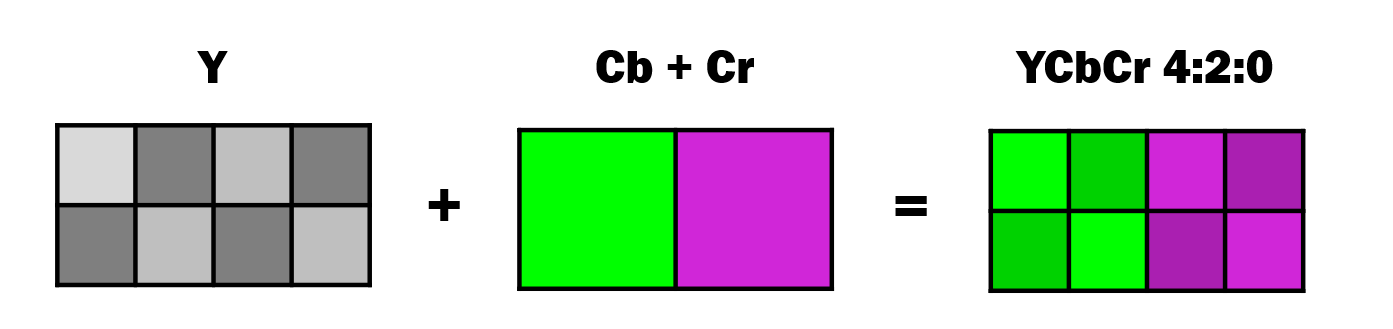
\includegraphics[width=0.8\textwidth]{res/yuv420.png}
	\caption{4:2:0 chroma subsampling. The 4 refers the width of the grid, which has (fixed) height 2. The 2 specifies that the horizontal resolution is halved (two "horizontal" samples), while the 0 that there are no different samples between the first and the second row.}
	\label{fig:yuv420}
\end{figure}

When compared to a typical 8-bit RGB image (equivalent to Y'CbCr 4:4:4, i.e. no subsampling), requiring 24 bits per pixel, a Y'CbCr 4:2:0 image requires only 12 bits per pixel, resulting in a 50\% saving with very similar perceived quality. When using tools like \texttt{ffmpeg}, Y'CbCr 4:2:0 is often called \texttt{yuv420p} or similar.

\subsection{Inter-frame and intra-frame compression}
\label{sec:bg/compression/intra-inter}

All the main video coding standards released since the early 1990s are based on a \textbf{hybrid codec model} that exploits both temporal and spatial redundancy of videos to achieve high compression ratios.

Temporal compression, or \textbf{inter-frame compression}, relies on the fact that there is usually a high similarity between consecutive video frames. On the other hand, spatial compression, or \textbf{intra-frame compression}, takes advantage of the fact that pixels that are close to each other within a picture are usually highly correlated.

Video \textbf{codecs} (en\textbf{co}der/\textbf{dec}oder) are implementations of video coding standards that are able to convert the input video into a coded version in a way that is reversible, i.e. such that the decoder can reconstruct the original video with some approximation. Encoders should output a compressed representation that is as efficient as possible while trying to preserve the fidelity of the original video.

\begin{figure}[h]
	\centering
	
	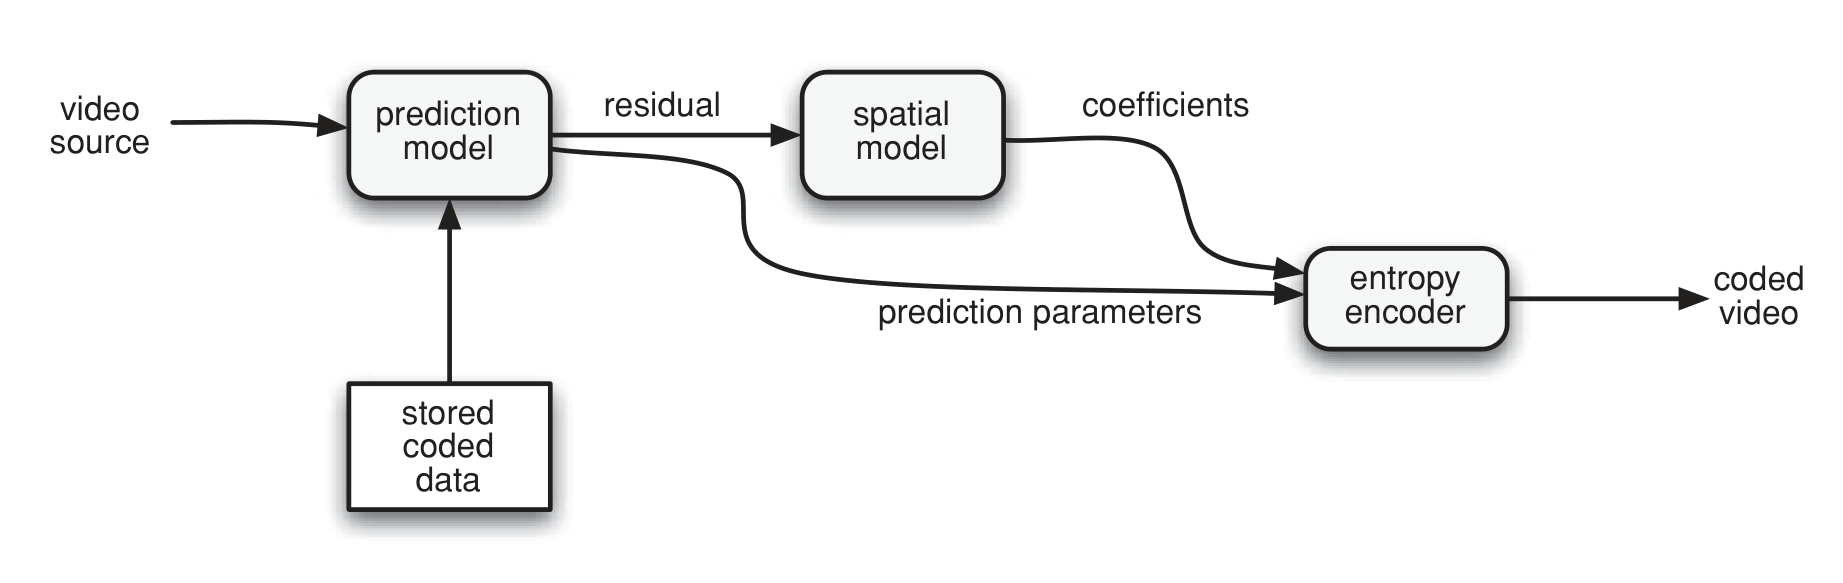
\includegraphics[width=\textwidth]{res/hybrid_codec_high_level.png}
	
	\caption{High-level hybrid codec architecture.\cite{h264}}
	\label{fig:codec_highlevel}
\end{figure}

In general, a hybrid video codec works in three phases:\cite{h264}

\begin{itemize}
    \item \textbf{Prediction model}: exploits spatial or temporal redundancy by producing a prediction of the current frame (or block of a frame) being analyzed. This is done by looking at a previous reference frame or at other parts of the same frame. The outputs of this phase are a \textbf{residual frame}, which is the difference between the actual frame and the predicted frame, and the parameters that define how the prediction was obtained. By encoding only the residual and the parameters we can basically store only the "error" of the prediction and greatly reduce the amount of data that needs to be coded. The prediction can be obtained in two ways:
        \begin{itemize}
            \item \textbf{Temporal prediction}: in its most basic form, the prediction is the difference between the current frame and a previous (or future) reference frame. In practice, we also need to take into account the motion that occurs between frames by running a \textbf{motion estimation} algorithm that for each block\footnote{Blocks are small regions of pixels.} in the current frame finds the best matching block in the reference frame. The \textbf{motion-compensated block} becomes the prediction used to calculate the residual, which becomes the output of the prediction phase together with the \textbf{motion vectors} that explain how the prediction block was obtained (i.e. how it "moved" with respect to the reference frame).
            \item \textbf{Spatial prediction}: when encoding a block of the image, a prediction of the pixel values of the block is first calculated by looking at neighboring pixels. Statistically, pixels close to each other are expected to be similar due to spatial redundancy. Usually, this step consists of looking at the pixels on the left and/or top edges of the block. The predicted block is then subtracted from the current block to obtain a \textbf{residual block}, which is passed on to the next phase together with the information that tells how the prediction of the block was obtained.
        \end{itemize}
        
    \item \textbf{Spatial model}: in most codecs, this phase consists in compressing the residual frame through a transform and quantization step, followed by the encoding of the obtained coefficients.
        \begin{itemize}
            \item The \textbf{transform} step often consists in applying the \textbf{Discrete Cosine Transform} (DCT) to transform the blocks from the space to the frequency domain. The output of the DCT is a matrix of coefficients, which can be used to faithfully reconstruct the original block, although without achieving any compression.
            \item In the \textbf{quantization} step, coefficients that have insignificant impact, such as values that are close to zero, are discarded, enabling to represent the original block with some approximation by storing a smaller number of DCT coefficients (the non-discarded ones). In the decoder, the subset of coefficients can then be fed into the \textbf{IDCT} (the inverse of the transform), obtaining a reconstruction of the original block. The fidelity of the reconstruction depends on how strong the quantization step was, that is in practice on the \textbf{quantization parameter} (QP).
            \item After quantization, the remaining coefficients are reordered through a \textbf{zigzag scan} of the matrix, so that the most significant coefficients will be at the beginning of the sequence (a typical property of the DCT), and then encoded through \textbf{Run-Level Encoding} (RLE).
        \end{itemize}
     
    \item \textbf{Entropy coding}: in this phase, all the information collected in previous phases, including quantized coefficients, quantization parameters and motion vectors, is encoded in a bit stream. To exploit the statistical redundancy of symbols in the data, techniques like \textbf{Variable-Length Coding} (VLC), such as Huffman coding, or arithmetic coding and \textbf{Context-aware Arithmetic Encoding} (CAE) are used, achieving further compression.
\end{itemize}

\begin{figure}[hb]
	\centering
	
	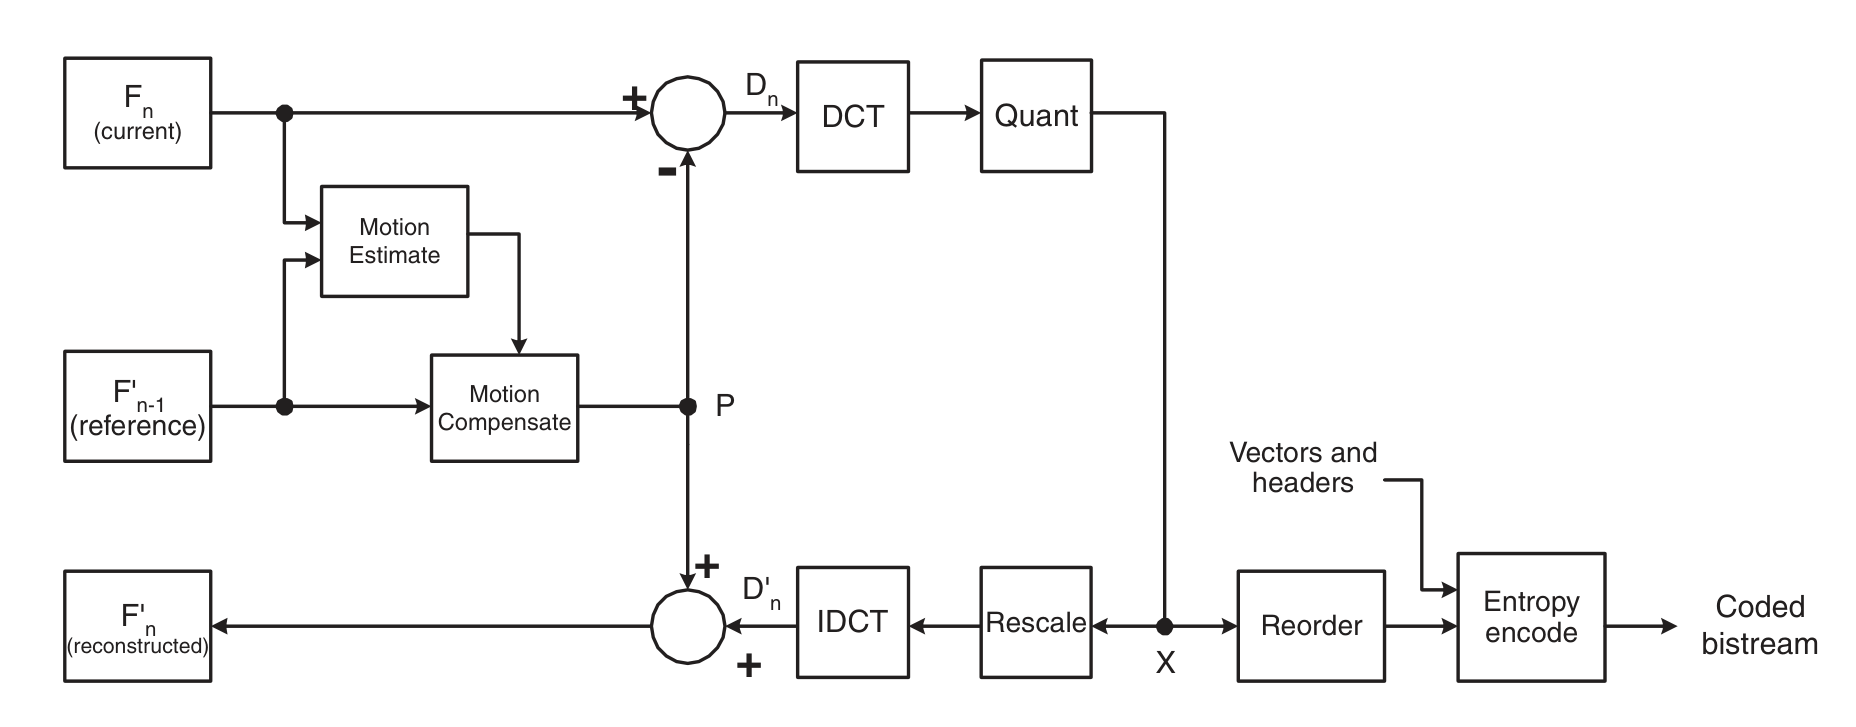
\includegraphics[width=\textwidth]{res/hybrid_codec_detailed.png}
	
	\caption{Detailed hybrid codec architecture.\cite{h264}}
	\label{fig:codec_detailed}
\end{figure}

%The transform converts the samples into another domain in which they are represented by transform coefficients. The coefficients are quantized to remove insignificant values, leaving a small number of significant coefficients that provide a more compact representation of the residual frame. The output of the spatial model is a set of quantized transform coefficients.

%The parameters of the prediction model, i.e. intra prediction mode(s) or inter prediction mode(s) and motion vectors, and the spatial model, i.e. coefficients, are compressed by the entropy encoder. This removes statistical redundancy in the data, for example representing commonly occurring vectors and coefficients by short binary codes. The entropy encoder produces a compressed bit stream or file that may be transmitted and/or stored. A compressed sequence consists of coded prediction parameters, coded residual coefficients and header information. The video decoder reconstructs a video frame from the compressed bit stream. The coefficients and prediction parameters are decoded by an entropy decoder after which the spatial model is decoded to reconstruct a version of the residual frame. The decoder uses the prediction parameters, together with previously decoded image pixels, to create a prediction of the current frame and the frame itself is reconstructed by adding the residual frame to this prediction.

The output of a hybrid video encoder is a \textit{bit stream} (or \textit{bitstream}), namely a compressed sequence of coded residual coefficients and other parameters. The decoder applies the same process inversely to reconstruct the original video frames, with some approximation.

\subsection{Frame types and GOP}
\label{sec:bg/compression/gop}

As we have seen, the prediction model can be based on temporal (inter-frame) prediction or spatial (intra-frame) prediction. The type of prediction that is used and which reference frames are used for the prediction determine the type of frame. In particular:

\begin{itemize}
    \item \textbf{I-frames} (\textit{Intra-frames}) are frames that do not require any other frames to be decoded and are thus compressed only by intra-frame prediction.
    \item \textbf{P-frames} (\textit{Predicted frames}) are frames that can reference other previous frames when performing temporal prediction. Depending on the codec, a frame can reference one or more previous frames.
    \item \textbf{B-frames} (\textit{Bi-directional predicted frames}) are frames that can reference both previous and future frames as reference frames in temporal prediction. They are more computationally expensive to encode, but are usually the most compressible ones.
\end{itemize}

Because of inter-frame dependencies, the display order of frames is very often different from the decoding order. For this reason, in codecs jargon there is the distinction between Presentation Time Stamps (PTS), and Decode Time Stamps (DTS).

Depending on the type of frames that are used to encode a video sequence, different \textbf{prediction structures} can be obtained. For example, low delay applications could use a structure like the one in figure \ref{fig:codec_gop1}, where only I-frames and P-frames are used and P-frames always reference the previous frame. I-frames should be inserted into the stream periodically to allow more efficient random access (\textit{seeking}). Another reason is that in some cases scene cuts might justify the use of an I-frame instead of a P-frame, depending on how drastic the scene change is.

\begin{figure}
	\centering
	
	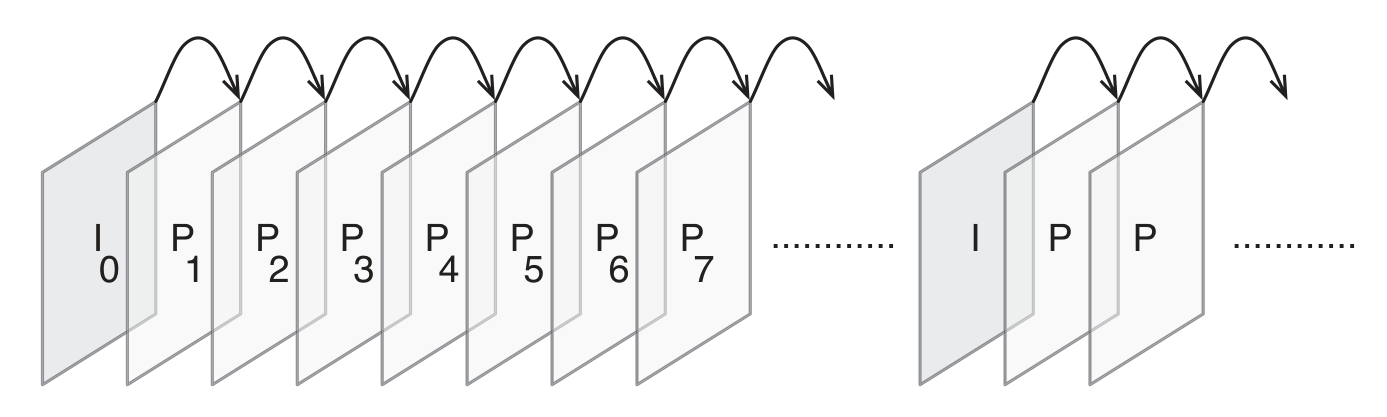
\includegraphics[width=0.9\textwidth]{res/gop1.png}
	
	\caption{Simple GOP structure with no B-frames.}
	\label{fig:codec_gop1}
\end{figure}

Most of the time, the arrangement of the frames is much more complex and is usually defined by a \textbf{Group of Pictures (GOP)} structure, as seen in Figure \ref{fig:codec_gop2}. A GOP always starts with an I-frame and is most of the time \textit{closed}, which means that it is independent from previous and future GOPs. As a consequence, in a closed-GOP scenario the decoder does not need access to previous of future GOPs to be able to decode frames in the current GOP.

The structure of a GOP can be summarized as a string sequence, like \texttt{IBBPBBPBBPBBI}, or through two numbers, \texttt{M} and \texttt{N}, that respectively determine the distance between P-frames, and the GOP size. For example, the structure in Figure \ref{fig:codec_gop2} can be expressed as \texttt{M=3, N=12}.

\begin{figure}
	\centering
	
	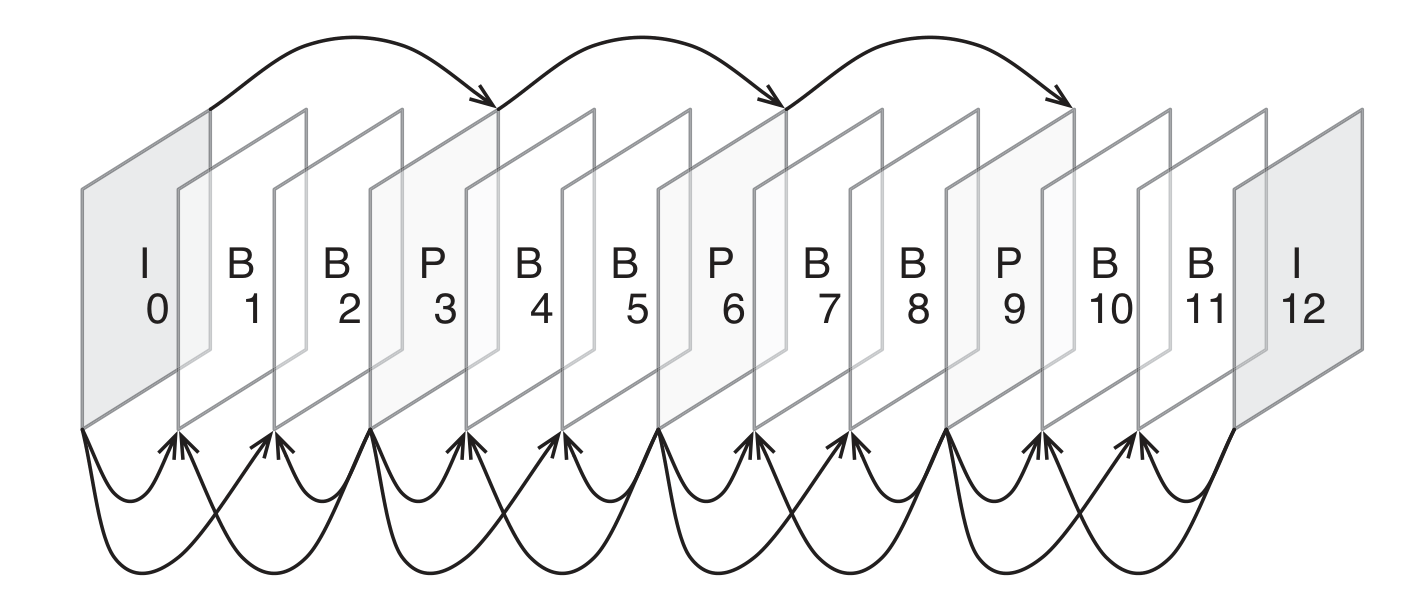
\includegraphics[width=0.8\textwidth]{res/gop2.png}
	
	\caption{Typical GOP structure, \texttt{M=3, N=12}.}
	\label{fig:codec_gop2}
\end{figure}

\subsection{Popular video coding formats}
\label{sec:bg/compression/codecs}

The dominant video coding standard is currently \textbf{H.264}, sometimes referred to as \textit{Advanced Video Coding} (AVC) or \textit{MPEG-4 Part 10}, developed by a joint team of the ITU (Video Coding Experts Group) and ISO (Moving Picture Experts Group, or \textbf{MPEG}). H.264 was first standardized in 2003, nevertheless it is estimated that H.264 is still used today by more than 80\% of the companies in the industry, thanks to its good performance (both in terms of compression and encoding/decoding efficiency) and the accessible royalties structure.\cite{bitmovin}

It is worth noting that the H.264 standard only defines the format and syntax of the H.264 bitstream and how to decode it, but it does not specify how to actually encode a video. Therefore, the term \textit{codec} should only be used to refer to the actual implementations of H.264, which typically include both an encoder and a decoder.

The successor of H.264, first published in 2013, is \textbf{H.265}, also named \textit{High Efficiency Video Coding} (HEVC) or \textit{MPEG-H Part 2}, which provides better compression of 25\% to 50\% better compression at the same bitrate compared to H.264. It is especially suitable for high-resolution content such as 4K UHD, but struggled to reach wide adoption due to the complex and expensive royalties structure that slowed down hardware support.\cite{hevcroyalties}

In competition with the H.26x family of formats, Google released royalty-free \textbf{VP8} in 2008, followed by \textbf{VP9} in 2012. Thanks to Google controlling a large fraction of the browser market share and the YouTube streaming platform, VP9 became a popular alternative to H.264, often delivering better video compression ratios with comparable quality.

% TODO: sources

The successor to VP9 was incorporated into \textbf{AV1} (first released in 2018), the royalty-free video format developed by the \textit{Alliance for Open Media} (AOMedia), an initiative backed by large companies such as Google, Apple, Meta, Microsoft, Amazon, Netflix, Cisco, NVIDIA, Intel, among others.\footnote{\url{https://aomedia.org/membership/members/}} AV1 is much more complex than H.264 and achieves up to 50\% better compression when compared to H.265, making it especially suitable for high-resolution content such as 4K UHD or 8K UHD. The downside of AV1 is that since it is quite complex, codec implementations are often prohibitively expensive to run in software, thus requiring hardware support. However, having widespread hardware support is an effort that can take quite a few years.\cite{av1}

\subsubsection{H.264}
\label{sec:bg/compression/codecs/h264}

\begin{figure}
	\centering
	
	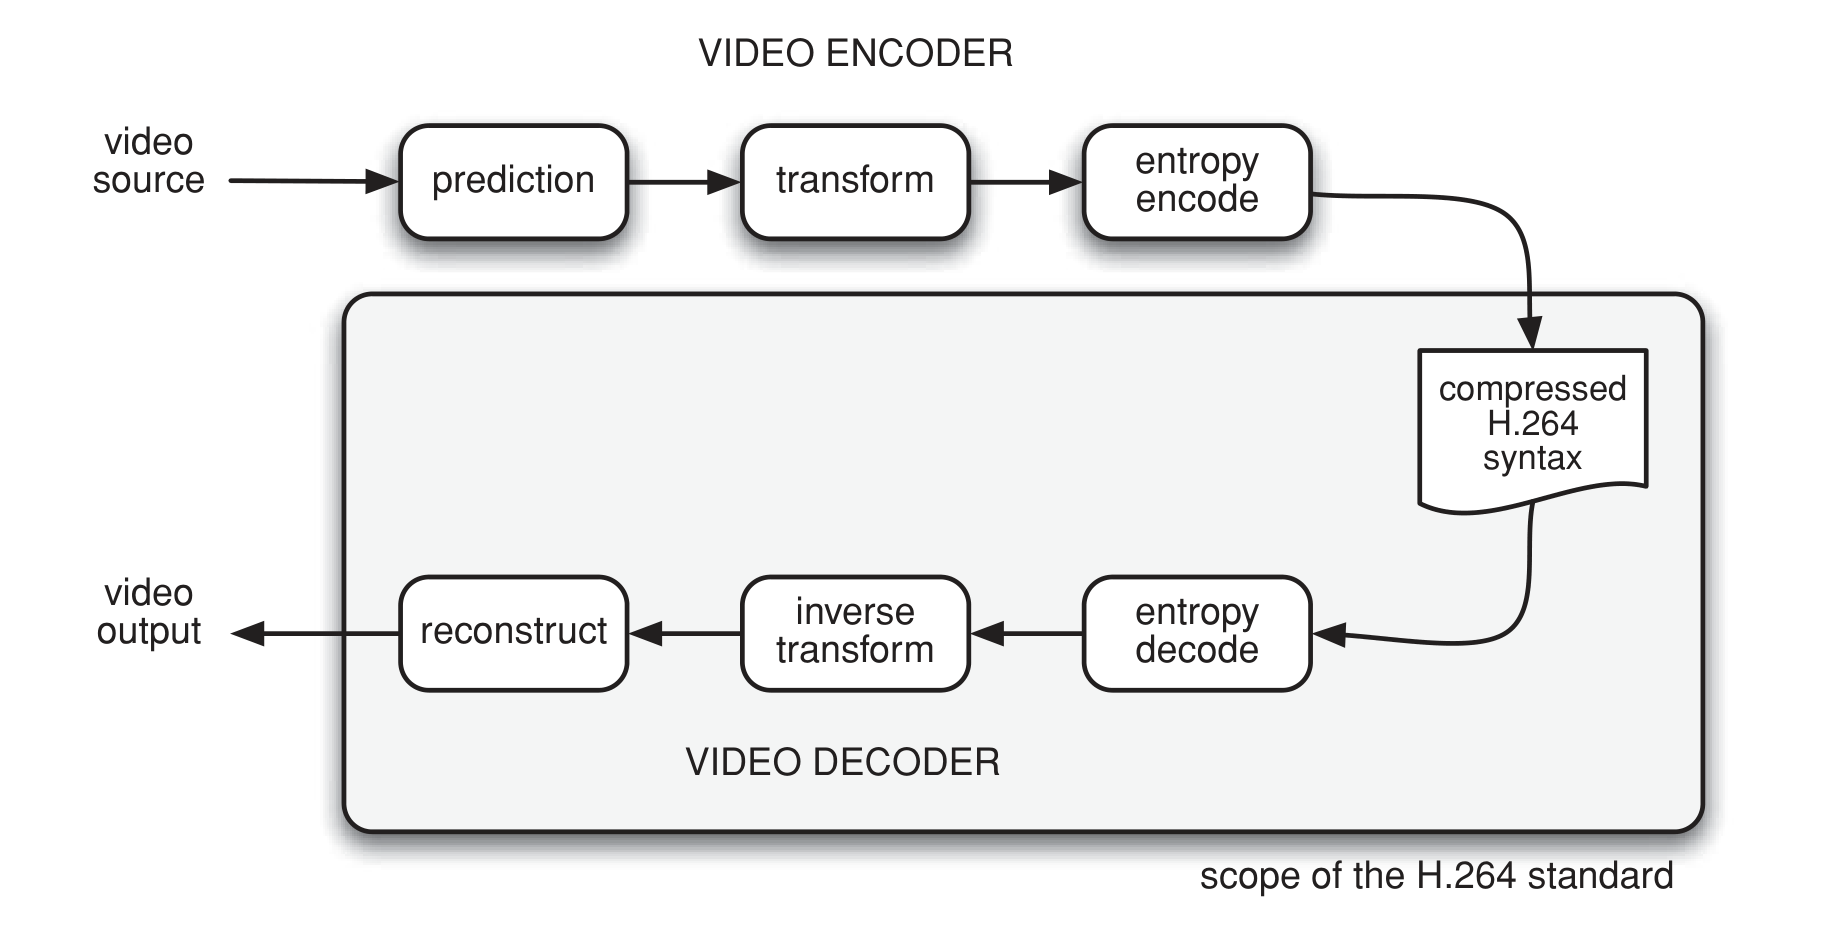
\includegraphics[width=0.8\textwidth]{res/h264_scope.png}
	
	\caption{The scope of the H.264 standard.}
	\label{fig:h264_scope}
\end{figure}

As we have seen, H.264 is still the dominant video format in the industry. Since the standard covers only the decoding part of the codec, as shown in Figure \ref{fig:h264_scope}, many codec implementations have been released, achieving different compression results. One of the most popular H.264 encoders is \texttt{x264}, which is open source and software-based, typically scoring as the best speed/quality trade-off in H.264 codec comparisons.\cite{msu2021} \texttt{x264} is also the default codec in \texttt{ffmpeg}, a very popular tool for video and audio manipulation and compression.

H.264 is based on the hybrid codec model we have introduced earlier. In H.264, video frames are divided into 16x16 pixels \textbf{macroblocks} (MB), on which the prediction model is applied. Macroblocks can be split into partitions that can be as small as 4x4 pixels (not necessarily square), so that the same macroblock can reference different macroblocks, possibly in different reference frames.

In H.264, the transform is an approximation of the DCT and can be applied on 4x4 or 8x8 blocks. Quantization can be controlled by the QP parameter, or step size, which ranges from 0 to 51 and is usually adjusted automatically by the encoded depending on the input configuration. Finally, for the entropy coding step, H.264 supports both variable-length coding and arithmetic coding techniques.

As not every device is capable of supporting all features of the standard, H.264 includes the concept of profiles and levels. A \textbf{profile} defines the H.264 features the decoder must support to be able to decode the compressed video. Common profiles are: the baseline profile, which does not include support for B-slices\footnote{In H.264 the concept of I-frames, P-frames and B-frames is replaced by the slices equivalent. A slice is a subset of macroblocks contained in a video frame.} or CABAC\footnote{Context-aware Arithmetic Coding.}; the main profile, which supports both B-slices and CABAC; the high profile, which includes additional optimizations such as adaptive selection of the block size for the transform step. The \textbf{level} instead specifies an upper limit on frame size, decoding rate, and memory required to decode the video.

Finally, an important part of H.264 is the syntax of the coded bitstream. The H.264 data is organized into a sequence of packets known as \textbf{Network Abstraction Layer Units} (NAL units or \textbf{NALUs}). Since units can be of varying length, there should be a way to distinguish when a unit ends and the next one begins. There are mainly two approaches to solve this problem:

\begin{itemize}
    \item Transporting NAL units by wrapping them in \textbf{packets}, which could be network packets or a structure defined by the \textbf{container format}, as we will see in the following sections.
    \item Treating the coded bitstream as a \textbf{byte stream}. In this case, a \textit{start code}, a 3-byte sequence that acts as a synchronization marker, is inserted before each NAL unit so that the decoder can identify the boundaries of the units. This byte stream format is defined by the \textit{Annex B} of the standard, which is the reason why this format is very often referred to as \texttt{annexb}.
\end{itemize}

\begin{figure}
	\centering
	
	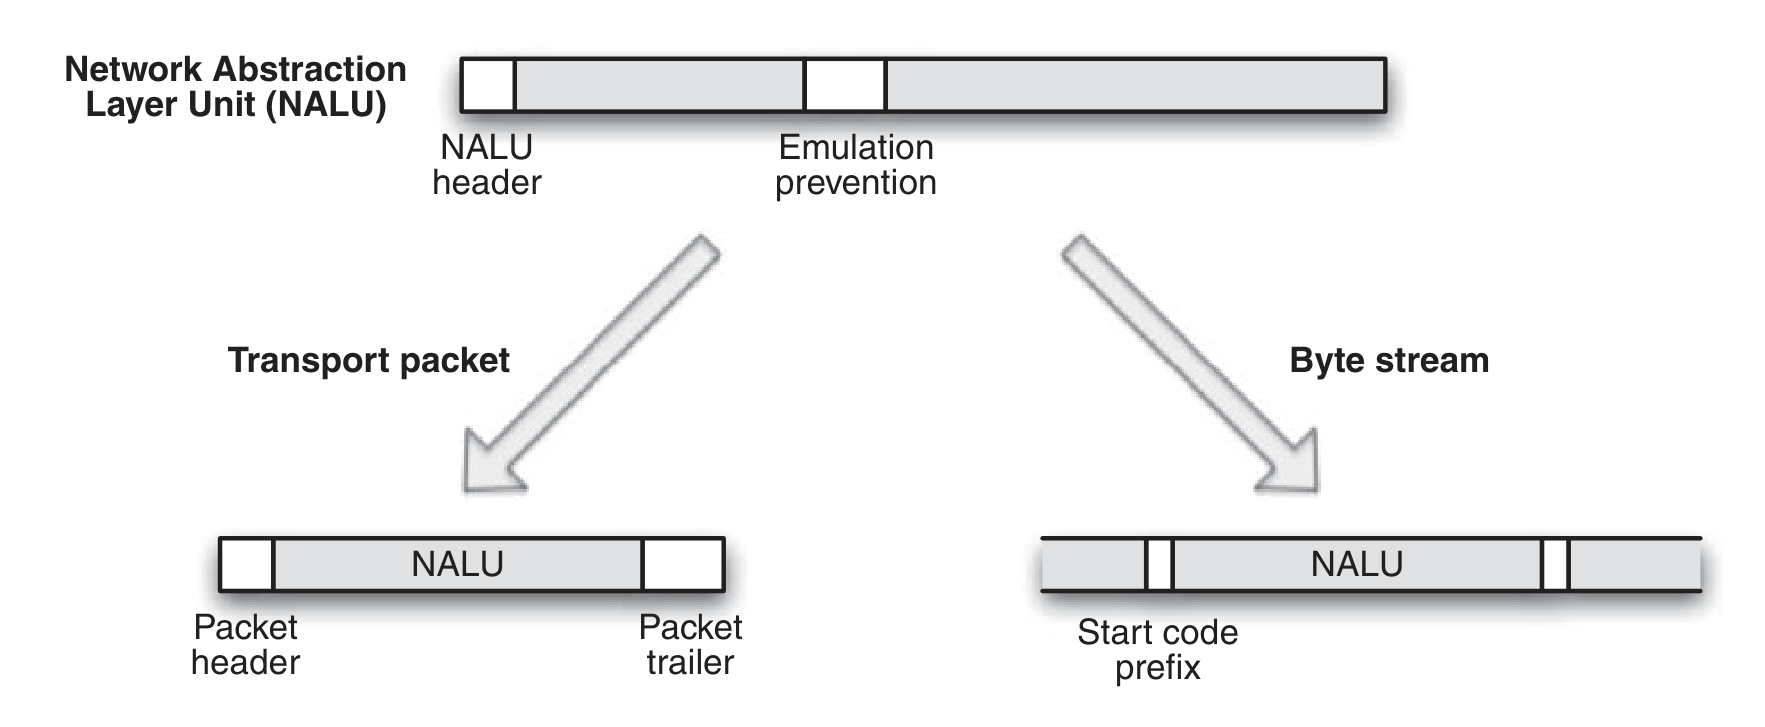
\includegraphics[width=0.9\textwidth]{res/h264_nalu.png}
	
	\caption{H.264 bitstream structure and encapsulation alternatives.}
	\label{fig:h264_encapsulation}
\end{figure}

\section{Digital audio and compression}
\label{sec:bg/audio}

Digital audio is generally represented through the \textbf{Pulse Code Modulation} (PCM) method, which is characterized by two main parameters: \textbf{sample rate}, which defines how frequently the sound level was measured when captured from the analog domain, and \textbf{bit depth}, which refers to the number of bits used to store a sample.

Although uncompressed PCM audio is more tractable than video, since it is much lighter (a stereo audio track with 44.1 kHz sample rate and 16-bit samples requires "only" 1.4 Mbps), audio is typically highly compressible since human sound perception is limited. Audio coding formats such as \textbf{MP3} and \textbf{AAC} are based on perceptual coding, as they tend to discard sound information that would otherwise be inaudible and can achieve excellent quality with savings of up to 90\%.\cite{aac}

\textbf{AAC} is nowadays the most widely used audio format in streaming scenarios and is supported by virtually every device.\cite{bitmovin} AAC comes in multiple variants, with \textbf{Low Complexity} (AAC-LC) being the most common, as it is widely supported and provides good compression ratios and quality. Other common versions are those of the \textbf{High Efficiency} (HE) family, which are optimized for low-bitrate applications.

In the AAC bitstream, audio samples are organized into packets that contain a fixed number of samples, typically 1024. To reduce compression artifacts, AAC uses a modified version of the DCT transform that works with overlapping samples. This means that, in practice, for each AAC packet encoded or decoded another packet with the same number of samples is required. For this reason, AAC encoders add at least 1024 silence samples before the first actual audio sample, a technique called \textbf{priming}. Since this delay could introduce synchronization problems when audio is combined with video, decoders need to detect priming and correctly take into account the encoder delay.\cite{aacpriming}

\section{Container formats}
\label{sec:bg/containers}

Bitstreams produced by video and audio encoders often do not contain enough information to allow video players to actually play the video or audio file. For example, in H.264 the timing information is optional and without it the decoder does not know how to assign timestamps to individual video frames, or even determine the duration of the video.\cite{h264itu} In AAC, the raw frames do not contain information such as the sample rate or the variant of AAC used to encode the samples.\cite{aac}

\textbf{Container formats} solve this problem by wrapping the bitstreams in a structure that is common between different coding formats. Container formats also allow the grouping of multiple video, audio and subtitle tracks, an operation known as \textbf{muxing} (from \textit{multiplexing}) performed by \textbf{muxers}. Instead, the process of extracting tracks from a container format is known as \textbf{demuxing}.

Two popular container formats used in the context of video streaming are \textbf{MPEG-2 Transport Stream} and \textbf{MP4}.

\subsection{MPEG-2 Transport Stream}
\label{sec:bg/containers/mpeg2ts}

MPEG-2 Transport Stream (or \textbf{MPEG-2 TS}), defined by the MPEG-2 Part 1 standard, is a container format originally designed for digital television broadcasting systems. For this reason, it includes features such as error correction and synchronization, providing protection against degraded transmission channels.

A single MPEG-2 Transport Stream can transport multiple programs, for example multiple TV channels. Each program can consist of multiple video and audio streams, known as \textbf{elementary streams}. The coded data for each elementary stream is packetized into PES (Packetized Elementary Stream) packets, each having a fixed length of 188 bytes. The 188 bytes include headers (which transport data like timing information), which is the reason why Transport Stream often has a non-negligible overhead.\cite{mpeg2ts}

% terrible, rewrite
% https://tsduck.io/download/docs/mpegts-introduction.pdf

An H.264 bitstream muxed in an MPEG-2 stream must be in the Annex B format (i.e. with start codes).

\subsection{MP4 and fragmented MP4}
\label{sec:bg/containers/mp4}

MP4 is a container file format based on the \textbf{ISO Base Media File Format} (ISOBMFF). It was extended from Apple QuickTime File Format (\texttt{.mov}) and first published in 2001 as MPEG-4 Part 14.\footnote{The actual box structure is defined in MPEG-4 Part 12 (ISOBMFF).}\cite{mpeg4part12}

In the \textbf{ISOBMFF} format the video and audio bitstreams, such as an H.264-compressed video, are stored as tracks and organized in a \textbf{box structure}. The MP4 format is capable of storing metadata such as video duration and per frame display and decoding timestamps, dealing with issues such as synchronization between tracks and random access (\textit{seeking}) of the media file.

% Video and audio frames are usually interleaved, although it is possible to generate "flat" MP4 files where tracks are organized sequentially.

Some ISOBMFF box (or atom) types that are particularly relevant are:

\begin{itemize}
    \item \texttt{ftyp} (\textit{file type}), which includes some general information about the file type, e.g. the version of the MP4/QuickTime specification the file is compliant with.
    \item \texttt{moov} (\textit{movie header}), containing metadata about the tracks, such as the creation time, the duration, the resolution, the bitrate, the tables that allow players to quickly find the part of the file where a specific frame or timestamp can be found, etc.
    \item \texttt{mdat} (\textit{movie data}), containing the actual audio and video samples.
\end{itemize}

An H.264 bitstream muxed in an MP4 container does not need start codes and therefore must not be in the Annex B format. H.264 bistreams in MP4 files are stored in a format known as \texttt{avcC}, where the H.264 NAL units are preceded by their length.

A typical structure of an MP4 file consists of a \texttt{ftyp} box followed by a \texttt{moov} box (containing the tracks metadata), and finally the actual data stored in a \texttt{mdat} box. The \texttt{moov} box is sometimes placed at the end of the file, since the information required to create the box is often available only at the end of the encoding process.

For some use cases, such as adaptive video streaming, a more suitable structure is the one provided by the \textbf{fragmented MP4} format, or \textbf{fMP4}. In this format, the sequence is divided into fragments that can be transmitted and played independently. The structure of an fMP4 file still has \texttt{ftyp} and \texttt{moov} boxes at the beginning, shared among all fragments, while the rest of the file consists of a sequence of \texttt{moof} and \texttt{mdat} boxes, where the \texttt{moof} box contains metadata about the fragment, like the fragment index and the timestamp, and the \texttt{mdat} contains the video or audio samples for a single fragment (typically a few seconds of content).

\begin{figure}
	\centering
	
	\begin{subfigure}[t]{0.45\textwidth}
		\centering
		\begin{minted}[frame=single,fontsize=\small]{text}
[ftyp] size=8+16
  major_brand = isom
  minor_version = 1
  compatible_brand = isom
  compatible_brand = avc1
[moov] size=8+424781
  ...
  [trak] size=8+412772
  ...
  [trak] size=8+5742
  ...
  [trak] size=8+5718
  ...
[mdat] size=8+355431683
...
		\end{minted}
		\caption{MP4 file structure.}
		\label{fig:mp4dump_progressive}
	\end{subfigure}%
	~ 
	\begin{subfigure}[t]{0.45\textwidth}
		\centering
		\begin{minted}[frame=single,fontsize=\small]{text}
[ftyp] size=8+20
  major_brand = isom
  minor_version = 1
  compatible_brand = isom
  compatible_brand = avc1
  compatible_brand = iso5
[moov] size=8+1542
  ...
[moof] size=8+2088
  ...
[mdat] size=8+198008
  ...
[moof] size=8+2088
  ...
[mdat] size=8+198008
  ...
		\end{minted}
		\caption{Fragmented MP4 (fMP4) file structure.}
		\label{fig:mp4dump_fragmented}
	\end{subfigure}
	
	\caption{Comparison between MP4 and fMP4 file structures. Extracted with the \texttt{mp4dump} tool (Bento4).}
	\label{fig:mp4dump_progressive}
\end{figure}


\section{Adaptive bitrate technologies}
\label{sec:bg/abr}

In a typical live streaming architecture, we can generally distinguish three main parts: \textbf{ingestion}, \textbf{transcoding and packaging}, and \textbf{distribution}.

% TODO: architecture diagram

\textbf{Ingestion} refers to the process of making the input feed available to the transcoder server for processing. Often, this means having a client push the stream through an ingestion protocol such as \textbf{Real Time Messaging Protocol} (RTMP) or \textbf{Secure Reliable Transport} (SRT). In some cases, a more suitable approach is a pull-based one, where it is the backend system's responsibility to "pull" the video and audio streams from another system and pass them onto the pipeline.

Usually, the input feed is a high-bitrate/high-quality stream that is not suitable for streaming. The de facto standard for video streaming in the industry is \textbf{Adaptive Bitrate Streaming} (ABR) or \textbf{HTTP Adaptive Streaming} (HAS), which is based on the idea of producing multiple video renditions in advance on the server side, each of them having different encoding parameters, such as video resolution, framerate, and most importantly average/peak bitrate. The aim is to provide the client with the best video variant according to the estimated network throughput. The two main ABR protocols are \textbf{MPEG-DASH} and \textbf{Apple HLS}, as we will see in detail.

In order to allow clients to switch to a different video rendition when network conditions change, video files are split into small segments with a fixed duration that is usually between 4 and 10 seconds. At each segment boundary, the client can choose to switch to a different quality level by simply starting to download video segments of another rendition. The strategy that determines which video quality level to request is usually implemented on the client side by making use of \textbf{rate adaptation algorithms}.

Video segment files can be generated statically and published on a web server (\textbf{static packaging}) or dynamically generated on the fly (\textbf{dynamic packaging} or Just-In-Time packaging). The packaging step is performed by a \textbf{packager}, or segmenter, which also produces the metadata that allows the client to obtain the list of video renditions (identified by their bitrate and other encoding parameters) and the list of segment files for each rendition. In MPEG-DASH, there is a single-file manifest containing this information, while with HLS there are multiple playlist files.

It should be noted that the video and audio files produced by this step need to be in a coding and container format compatible with the adaptive bitrate technology chosen. For example, MPEG-DASH (see Section \ref{sec:bg/technologies/dash}) requires streams to be muxed in a fragmented MP4 container. Also, for best performance, the segments should start with an I-frame, so that the player can switch between renditions at segment boundaries. For this reason, the GOP size of the renditions should match the length of the segment. Another important thing to take into account is the bitrate, which should not oscillate too much so that the bitrate adaption algorithms can use the average bitrate as a reference value to make decisions.\cite{ozer}

Although ABR streaming is a generic term for adaptive bitrate technologies, most of the time segmented video and audio tracks and manifest files are delivered to the client through the \textbf{Hypertext Transfer Protocol} (HTTP). Using HTTP for \textbf{distribution} makes it easy for streaming platforms to scale, thanks to the widespread availability of \textbf{Content Delivery Networks} (CDN) and their global distribution networks. One of the important advantages of relying on CDNs is the possibility to cache video segments at the edge of the networks, as close as possible to the final users, therefore reducing latency and probability of congestion.

Also, transporting video traffic over HTTP instead of, for example, UDP avoids issues with firewalls and is, in general, highly reliable since video becomes normal HTTP traffic. Apart from scalability, mentioned above, this approach makes it possible to take advantage of important HTTP features, such as HTTPS for secure communication.

\subsection{Apple HTTP Live Streaming (HLS)}
\label{sec:bg/abr/hls}

HTTP Live Streaming (HLS) is an adaptive streaming protocol based on HTTP designed by Apple. First introduced in 2009 and later standardized as RFC 9216, it is estimated to be the most popular streaming protocol, with more than 73\% video developers using it.\cite{rfc8216}\cite{bitmovin} The reason for this is not only the fact that HLS is the only HAS protocol that can be used on Apple mobile devices, but also the simplicity of the protocol.

HLS uses the \textbf{extended M3U format} (\texttt{.m3u8} extension) to define a set of playlists that contain information such as the list of streams or the list of segments for a particular stream. In particular, a \textbf{master playlist} provides a set of variant streams\footnote{In the HLS RFC, the terms \textit{variant} and \textit{rendition} have different meanings. We will use the term \textit{variant} in this section to adhere to the RFC, while using the two terms interchangeably in the rest of the thesis.}, each of which is a different version of the same content, usually differing by bitrate and other encoding parameters. Players download the master playlist at the beginning of the playback session and use the information contained in it to adapt to network conditions by switching between variants. An example of a master playlist is shown in Figure \ref{fig:hls_master}.

\begin{figure}[h]
    \centering
    \begin{minted}[frame=single]{text}
#EXTM3U
#EXT-X-STREAM-INF:BANDWIDTH=1280000,AVERAGE-BANDWIDTH=1000000
low.m3u8
#EXT-X-STREAM-INF:BANDWIDTH=2560000,AVERAGE-BANDWIDTH=2000000
mid.m3u8
#EXT-X-STREAM-INF:BANDWIDTH=7680000,AVERAGE-BANDWIDTH=6000000
high.m3u8
#EXT-X-STREAM-INF:BANDWIDTH=65000,CODECS="mp4a.40.5"
audio-only.m3u8
    \end{minted}
	\caption{Example of a HLS master playlist with variants. The first three variants contain both video and audio, while the fourth variant is audio-only. The first variant, corresponding to the \texttt{low.m3u8} media playlist, is defined with an average bitrate of 1000 kbps and a peak bitrate of 1280 kbps.}
	\label{fig:hls_master}
\end{figure}

When players want to play a specific variant, they load the \textbf{media playlist} corresponding to the variant. A media playlist must specify the maximum duration of the segments in seconds, followed by a list of \textbf{media segments}, characterized by their duration and URI (relative or absolute). In the case of on-demand content, the media playlist must contain the full list of segments that make up the video or audio file, while in the case of live streams, the playlist may include only a sliding window of segments. An example of a media playlist is shown in Figure \ref{fig:hls_media}.

\begin{figure}[h]
    \centering
    \begin{minted}[frame=single]{text}
#EXTM3U
#EXT-X-TARGETDURATION:6
#EXT-X-VERSION:3
#EXTINF:6,
segment-1.ts
#EXTINF:6,
segment-2.ts
#EXTINF:3,
segment-3.ts
#EXT-X-ENDLIST
    \end{minted}
	\caption{Example of a simple HLS VoD media playlist with three segments and a segment target duration of 6 seconds.}
	\label{fig:hls_media}
\end{figure}

The HLS media segments can be muxed into the MPEG-2 TS format (\texttt{.ts} files) or in the fragmented MP4 format (\texttt{.mp4} or \texttt{.m4s} files). The supported video codecs are H.264 and H.265. When using \texttt{fMP4} as the container format, media playlists must specify an \textbf{initialization segment} containing the \texttt{ftyp} and \texttt{moov} boxes with the \texttt{\#EXT-X-MAP} tag.

In addition to the RFC, Apple maintains an \textit{Authoring Specification for Apple Devices} defining additional rules for HLS streams, which are often taken as "safe" practices in the industry when producing content for adaptive bitrate streaming.\cite{hlsauthoring}

The authoring specification provides a set of recommendations to ensure compatibility with HLS implementation that can be found on Apple devices, including the following:

\begin{itemize}
    \item A table with a possible set of variants with their bitrate and frame rate (a \textit{bitrate ladder}), for both H.264 and H.265, plus a recommendation to adjust them according to the specific use case.
    \item An indication that the peak bitrate should be no more than 200\% of the average bitrate, although it is often recommended to make the bitrate as constant as possible.\cite{ozer}
    \item A recommendation for a segment duration of 6 seconds, although 4 seconds or lower are common values in practice.\cite{ozer}
\end{itemize}

HLS also includes support for encryption, ads, trick play (scrubbing and fast forward), subtitles, and multiple audio tracks.

There is a variant of HLS, known as \textbf{Low-Latency HLS} (LL-HLS), which is designed for low-latency live streaming. It is based on a technique called \textit{Blocking Preload Hints}, which relies on the fact that segments are made available in smaller parts called partial segments, which are published as soon as possible and can thus be downloaded before the full segment is made available. The HLS manifest now contains a "hint" about which partial segment should be requested next, so that the client can send the HTTP request before the partial segment is actually available. The server will “block” and respond with the part as soon as it is available. LL-HLS has a mandatory requirement for HTTP/2, therefore we did not take into consideration for the work in this thesis, which focuses on HTTP/3.

\subsection{MPEG Dynamic Adaptive Streaming over HTTP (DASH)}
\label{sec:bg/technologies/dash}

MPEG Dynamic Adaptive Streaming over HTTP (DASH) is an alternative to HLS for adaptive streaming over HTTP. It was developed by the MPEG group and first published in 2012. Since it is the officially supported ABR protocol on HbbTV, the entertainment system for smart TV, it gained popularity and is often mandatory for streaming platforms that want to target TVs. It is not supported on iOS and Apple TV, so HLS is often still an easier choice to ensure broad compatibility.

DASH is a very complex standard, so we will just give a broad overview of how it works.\cite{dash}\cite{dash2} The are several differences between HLS and DASH:

\begin{itemize}
    \item Unlike HLS, DASH is codec-agnostic, therefore it can be used with any codec without waiting the standard to be updated.
    \item It uses the \texttt{fMP4} container format by default, thus reducing the overhead introduced by MPEG-2 TS.
    \item DASH does not use M3U playlists: there is a single manifest file (\texttt{.mpd} extension) in XML format.
\end{itemize}

The manifest file has a nested structure that combines the equivalent of the master and media playlists of HLS. The main elements in a DASH manifest file are:\footnote{\url{https://www.brendanlong.com/the-structure-of-an-mpeg-dash-mpd.html}}

\begin{itemize}
    \item \textbf{Adaption sets}: they define a group of representations (renditions) on which adaptation algorithms are executed. A common approach is to have one video adaptation set and multiple audio adaptation sets depending on the number of supported audio languages.
    \item \textbf{Representations}: they represent the individual renditions in an adpatation set. Each representation usually has different encoding parameters, such as the bitrate, resolution and framerate, but could also have different codecs.
    \item \textbf{Media segments}: within a representation, there are multiple ways to specify how the player should obtain the media segments. For example, with \texttt{SegmentList} we can insert the full list of segments in the manifest file. A smarter approach is to use the \texttt{SegmentTemplate} element, which allows the packager to define a pattern for predictable sequences of segments.
    \item \textbf{Index segments}: they are the equivalent of the initialization segment, introduced with HLS.
\end{itemize}

A minimal example of a DASH manifest file is shown in Figure \ref{fig:dash_manifest}. In this case, there are two adaptation sets, one for video and one for audio. The video adaptation set contains two representations, corresponding to 720p and 540p. The file names of the segments are determined on the fly by the player using the \texttt{SegmentTemplate} definition. A similar approach is used for the audio adaptation set.

\begin{figure}[h]
    \centering
    \begin{minted}[frame=single,fontsize=\small]{xml}
<?xml version="1.0" encoding="utf-8" ?>
<MPD xmlns="urn:mpeg:dash:schema:mpd:2011" profiles="urn:mpeg:dash:profile:full:2011"
     type="static" mediaPresentationDuration="PT60S">
    <Period>
        <!-- Video -->
        <AdaptationSet id="0" mimeType="video/mp4" segmentAlignment="true"
                       startWithSAP="1" maxWidth="1280" maxHeight="720">
            <SegmentTemplate timescale="1000" duration="2000" startNumber="1"
                             initialization="$RepresentationID$/init.mp4"
                             media="$RepresentationID$/seg-$Number$.m4s" />
            <Representation id="720p" codecs="avc1.64001F" width="1280" height="720"
                            scanType="progressive" frameRate="25" bandwidth="3301246" />
            <Representation id="540p" codecs="avc1.64001F" width="960" height="540"
                            scanType="progressive" frameRate="25" bandwidth="2409696" />
        </AdaptationSet>
        <!-- Audio -->
        <AdaptationSet mimeType="audio/mp4" startWithSAP="1" segmentAlignment="true">
            <SegmentTemplate timescale="1000" duration="2000" startNumber="1"
                             initialization="$RepresentationID$/init.mp4"
                             media="$RepresentationID$/seg-$Number$.m4s" />
            <Representation id="audio" codecs="mp4a.40.2" bandwidth="131632"
                            audioSamplingRate="48000">
                <AudioChannelConfiguration
                    schemeIdUri="urn:mpeg:mpegB:cicp:ChannelConfiguration"
                    value="2" />
        </Representation>
        </AdaptationSet>
    </Period>
</MPD>
    \end{minted}
    \caption{A minimal example of an MPEG-DASH manifest files, showing two adaptation sets (video and audio). The video set contains two representations, 720p and 540p.}
    \label{fig:dash_manifest}
\end{figure}

In the example of Figure \ref{fig:dash_manifest}, the \texttt{type} field is set to \texttt{static}, which means that this manifest is for on-demand content. In the case of a live stream, the \texttt{type} has value \texttt{dynamic} and some additional fields are required. For example, the \texttt{availabilityStartTime} field specifies the timestamp corresponding to the start of the live stream, and is used by the player to calculate which segment should be requested next. Another important field is the \texttt{suggestedPresentationDelay}, which determines the target live latency (which can be overridden by the player).

The MPEG-DASH standard also has an extension for low-latency streaming, known as \textbf{Low-Latency DASH} (LL-DASH). The approach of LL-DASH is conceptually similar to that of LL-HLS, but is technically implemented in a different way. Specifically, it takes advantage of the \textit{Chunked Transfer Encoding} (CTE) feature of HTTP/1.1. Similarly to LL-HLS, LL-DASH makes use of chunks which can be downloaded as soon as they are published. The client sends a single HTTP request per segment and waits for chunks to be delivered through HTTP CTE, decoding and playing them as soon as possible. Compared to LL-HLS, LL-DASH has a smaller overhead since it sends a much lower number of HTTP requests.\cite{llhls_vs_lldash}

\subsection{Common Media Application Format (CMAF)}
\label{sec:bg/technologies/cmaf}

Before Apple introduced support for \texttt{fMP4} segments in 2016, a common issue for video platforms was that supporting both HLS and DASH required two copies of the same content, one in MPEG-2 TS format and the other in \texttt{fMP4}. This was needed because not all platforms support HLS and vice versa.

This problem led to the proposal and standardization of \textbf{Common Media Application Format} (CMAF), a common specification that defines how media should be packaged and segmented for delivery. Fragmented MP4 is a CMAF-compatible format and since it is supported by both HLS and DASH it can lead to significant savings. Video platforms can, in fact, produce and store a single set of video segment files and deliver them to all devices.\cite{cmaf}

\subsection{Media Source Extensions (MSE)}
\label{sec:bg/technologies/mse}

One of the main medium through which users watch video streams is web browsers. Apple includes native support for its HLS protocol in its own browser, Safari, which is pre-installed on all Apple devices (and is also the only browser engine that can be used on iOS). Other browsers typically do not include support for HLS and DASH, but instead support the \textbf{Media Source Extensions} (MSE) API, through which JavaScript libraries can implement HLS and DASH.\cite{mse}

MSE is a set of APIs that abstract the implementation of media playback in the browser. MSE exposes types and methods that allow the client-side code to push video and audio data for playback.

More in detail, MSE defines the \texttt{MediaSource} type as a source of media data for the \texttt{<video>} or \texttt{<audio>} HTML5 media elements, to which a \texttt{MediaSource} is attached. The client code interacts with the \texttt{MediaSource} to push new data, while the media elements fetch the data from the \texttt{MediaSource}.

\texttt{MediaSource} instances expose methods to attach a set of \texttt{SourceBuffer} objects, which represent individual media tracks like a video or audio streams. When new media data is available, such as a new video segments, the client calls the \texttt{appendBuffer()} method on the corresponding \texttt{SourceBuffer}, providing the new data for the track to the browser. The bytes of data must of course conform to the format set when creating the \texttt{SourceBuffer}, which must be supported by the browser. Most of the time this means the ISOBMFF (\texttt{fMP4}) or WebM container formats. Codec support instead often depends on the browser build/configuration and platform.

The libraries that implement HLS or DASH must take care of parsing the manifest files, downloading the segments, implementing rate adaption algorithms, potentially transmuxing from MPEG-2 TS to fragmented MP4 (such as with HLS), appending segment data to the source buffers while leaving the MP4 demuxing and stream decoding tasks to the browser.

In practice, this means that there can be many implementations of HLS and DASH, all relying on the Media Source Extensions underneath. For HLS, a popular implementation is \texttt{HLS.js}\footnote{\url{https://github.com/video-dev/hls.js/}}, while for DASH the official reference implementation is \texttt{dash.js}\footnote{\url{https://github.com/Dash-Industry-Forum/dash.js/}}. Several other JavaScript players include support for HLS and DASH, such as \texttt{Video.js}, \texttt{Shaka Player}, \texttt{THEOPlayer}, and \texttt{JW Player}, some of which are open source while others are commercial.

\section{Hypertext Transfer Protocol (HTTP) evolution}
\label{sec:bg/http}

When browsing the Web, we use an application layer protocol known as \textbf{Hypertext Transfer Protocol} or \textbf{HTTP}. In addition to being used for transferring HTML web pages and related files, we have seen that HTTP can be used by apdative streaming technologies to deliver video and audio segments to the client.

In this section, we will briefly go through three important versions of HTTP, their limitations, peculiarities, and how they are currently exploited by HLS and DASH for video streaming applications.

\subsection{HTTP/1.1}
\label{sec:bg/http1}

For a long time, the dominant HTTP version has been \textbf{HTTP/1.1}, first published in 1997.\cite{http1.1} It is based on the Transmission Control Protocol (TCP), the reliable connection-oriented transport layer protocol.

To send an HTTP request, a client should open a TCP connection with the server. It will then transmit the request line, followed by a list of headers, an empty line, and optionally a payload or message body. The following is an example of an HTTP/1.1 \texttt{GET} request to the URL \texttt{http://example.com/index.html}.

\begin{minted}[frame=single]{http}
GET /index.html HTTP/1.1
Host: example.com
User-Agent: curl
Accept: */*
\end{minted}

Once the server has received the request, it will do its processing and then start sending the response on the same TCP connection. The response consists of a status line, a list of headers, and optionally a message body, as in the following example.

\begin{minted}[frame=single]{http}
HTTP/1.1 200 OK
Date: Thu, 22 Dec 2022 08:00:00 GMT
Content-Type: text/html; charset=UTF-8

<html>
<head>
...omitted...
\end{minted}

For encrypted communication, HTTPS uses \textbf{Transport Layer Security} (TLS) to create a secure communication channel over TCP. The HTTP/1.1 request is then transmitted over the encrypted TLS session.

When keep-alive (persistent connections) is enabled, the same connection can be reused to send multiple HTTP requests, avoiding the overhead of establishing a new TCP connection and TLS session. HTTP/1.1 also supports request pipelining, meaning that multiple requests can be sent on the same TCP connection before receiving the responses, although it is rarely used because not all server implementations support it properly.

The main limitation of HTTP/1.1 is, however, that it does not support multiplexing of responses, meaning that responses must be transmitted sequentially by the server. This causes a problem known as \textbf{HTTP head-of-line blocking}, where the current request blocks the following requests. Browsers try to workaround this issue by opening multiple TCP connections to the same web server when loading web pages, up to a (configurable) limit.\footnote{For example, Firefox uses 6 as a default connection limit, but the value can be changed through the \texttt{network.http.max-persistent-connections-per-server} preference.} 

\subsection{HTTP/2}
\label{sec:bg/http2}

\textbf{HTTP/2}, published as a Proposed Standard in 2015 as RFC 7540, was an attempt to solve the main issues of HTTP/1.1, most notably the head-of-line blocking problem. At the same time, the aim of HTTP/2 was to use less network resources while reducing the perception of latency.\cite{http2}

In HTTP/2, clients establish a \textbf{single TCP connection} with the server. To allow requests and responses \textbf{multiplexing}, the protocol introduces a binary framing format in which requests and responses, which maintain the same HTTP semantics as in HTTP/1.1, are split into smaller units, known as frames. Frames can be interleaved, allowing multiple requests and responses to be transmitted in parallel. In order to identify to which request a frame belongs to, the concept of \textbf{streams} was introduced. Streams can be seen as virtual connections that are very light to create and generally correspond to single HTTP requests. Streams can also be reset, with the effect of immediately stopping the transmission of the associated data frames.

An important feature of HTTP/2 is \textbf{stream prioritization}. Since multiple streams can co-exist on the same TCP connection, there was the need for a mechanism to make better decisions on which stream goes first or is given priority. HTTP/2 allows clients to assign a \textbf{weight} between 1 and 256 to each stream, where a higher number means higher priority. In addition, clients can specify that a stream is dependent on another stream through its ID, effectively creating a \textbf{dependency tree}. The structure of the tree, and therefore the order in which requests are responded, is defined by the dependency relationships, while the division of resources between a set of "children" streams is determined by their weights.

The dependency tree approach of HTTP/2 is very flexible and allows clients to implement different \textbf{prioritization strategies}, with widely different performance results. In \cite{http2pri}, Wijnants et al. examined the behavior of the main browsers to determine which prioritization scheme they implemented. It turns out that only Mozilla Firefox chose to adopt a complex tree-based strategy. Google Chrome implements a much simpler sequential FCFS approach based on dynamic weights (giving more weight to requests deemed more important according to heuristics), Microsoft Edge (legacy) uses a naive round-robin strategy with no weights at all, while Safari follows a weighted round-robin scheme. Surprisingly, the experimental results showed superior performance when using the relatively simple strategy implemented by Chrome.

% TODO: diagrams
% https://speeder.edm.uhasselt.be/www18/files/h2priorities_mwijnants_www2018.pdf
% https://speeder.edm.uhasselt.be/www18/files/h2priorities_mwijnants_www2018_presentation.pdf
% https://speeder.edm.uhasselt.be/www18/
% https://quic.edm.uhasselt.be/files/fosdem.pdf
% https://youtu.be/nH4iRpFnf1c?t=440

In HTTP/2, the use of HTTPS is mandatory, making the protocol more secure by design. HTTP/2 also achieves better performance by compressing headers, thanks to the \texttt{HPACK} compression algorithm. Finally, a feature known as \textbf{HTTP/2 Server Push} allows the server to push additional unsolicited content in response to HTTP requests, theoretically reducing the need for additional round-trip times to request resources.

While all these features make sense, in practice HTTP/2 did not manage to provide the expected performance improvements, for multiple reasons:

\begin{itemize}
    \item The \textbf{Server Push} feature never really took off, with virtually no CDN having support for Server Push. Additionally, in 2022 Google removed Server Push support from Google Chrome, citing extremely low usage, almost no gain in performance, and complexities in browser implementation. Instead, it suggested developers to use the \textbf{preload hints} or \textbf{103 Early Hints} features, which are easier to use and can provide significant performance gains.\footnote{\url{https://developer.chrome.com/blog/removing-push/}}
    \item \textbf{Stream prioritization} was found to be inconsistently implemented by clients and servers, with a significant number of large CDNs apparently ignoring prioritization.\footnote{\url{https://github.com/andydavies/http2-prioritization-issues}} This led to the prioritization scheme of HTTP/2 being deprecated and replaced by a new mechanism at the same time HTTP/3 came out.
    \item When the \textbf{sequential prioritization strategy} is used, we get the same HTTP head-of-line blocking issue seen in HTTP/1.1, worsened by the fact that only a single TCP connection is used.
    \item The use of a single TCP connection leads to another problem known as \textbf{TCP head-of-line blocking}, where the bottleneck is not the HTTP design but TCP itself. In fact, while HTTP/2 multiplexes requests in multiple streams, at the transport layer TCP only sees a single opaque byte stream. As a consequence, TCP retransmissions delay the transmission of all streams and not just the one affected by packet loss. Additionally, TCP congestion control may reduce the throughput of the connection in case of congestion, affecting all the requests, while in HTTP/1.1 it is less likely that all the connections are affected at the same time.
\end{itemize}

\subsection{HTTP/3}
\label{sec:bg/http3}

To overcome the limitations of TCP-based approaches, the next version of HTTP, \textbf{HTTP/3}, was based on a new transport protocol called QUIC, which is built on top of the lightweight UDP. While HTTP/3 by itself does not introduce new features, the fact that it is based on a new protocol like QUIC allowed to rethink how a transport layer protocol should work from the ground up. QUIC was published as a Proposed Standard in May 2021 with RFC 9000, with HTTP/3 following in June 2022 as RFC 9114, after a few years of work.\cite{http3}

More in depth, the following are some main conceptual differences between HTTP/2 and HTTP/3:

\begin{itemize}
    \item Since QUIC is based on UDP, TCP features such as connection establishment, flow control, congestion control, and retransmissions are now implemented by QUIC.
    \item \textbf{TLS v1.3} is tightly integrated with QUIC, making security features such as encrypted communication mandatory. At the same time, this approach allows innovative features such as 1-RTT handshakes or 0-RTT session resumption to be seamlessly implemented, providing further performance improvements.
    \item Unlike TCP, QUIC provides a seamless \textbf{connection migration} feature that allows reuse of connections when the network connection changes.
    \item \textbf{Stream multiplexing} is moved "down" from the application layer to QUIC. HTTP/3 takes advantage of QUIC streams to provide request multiplexing. HTTP/3 clients or servers can cancel HTTP requests by \textbf{resetting} the underlying QUIC stream.
    \item HTTP/2 \textbf{stream prioritization} is replaced by a simpler priority mechanism, implemented at the HTTP/3 level. QUIC does not have stream prioritization.
\end{itemize}

% TODO: stack diagrams https://github.com/rmarx/h3-protocol-stack/blob/main/README.md

The \textbf{head-of-line blocking} issue caused by TCP in HTTP/2 is not present in HTTP/3, since streams are now a concept of the transport layer. Unlike TCP, in fact, QUIC does not see a single byte stream but multiple streams that can be treated independently (with respect to retransmissions, for example). However, if the scheduling strategy implemented by the server is sequential, there could still be head-of-line blocking because the slow transmission of a stream would block the other ones. The multiplexing scheduler depends on the server implementation and is often round-robin, according to the experiments run by Marx et al.\cite{quicdiversity}

The prioritization scheme used by HTTP/3 was introduced in RFC 9218, published together with HTTP/3, with the title \textit{Extensible Prioritization Scheme for HTTP}. As the title suggests, the new mechanism is actually not HTTP/3-specific and is defined for both HTTP/2 and HTTP/3. Clients that implement RFC 9218 can communicate their preferences on how the server should prioritize responses in two ways:\cite{rfc9218}

\begin{itemize}
    \item Through an HTTP header called \texttt{Priority}, in which the priority for the request is specified.
    \item Through a \texttt{PRIORITY\_UPDATE} frame, so that requests can be reprioritized after they have been sent. With HTTP/3, priority update frames are transmitted over a unidirectional QUIC stream dedicated to control commands.
\end{itemize}

The HTTP requests priorities defined by RFC 9218 are characterized by two parameters:

\begin{itemize}
    \item The \textbf{urgency} parameter (\texttt{u}), an integer value ranging from 0 to 7 in descending order of priority, with a default value of 3.
    \item The \textbf{incremental} parameter (\texttt{i}), indicating whether an HTTP response can be processed incrementally by the client, and therefore if it can benefit from being received concurrently. For example, the download of a standard JPEG image file would not benefit from being transmitted incrementally since the JPEG decoder usually needs the whole image to start decoding the picture. On the other hand, a CSS file could benefit from being delivered even partially if the browser is capable of interpreting the CSS rules before the whole file is downloaded. The default value of the incremental parameter is 0 (\texttt{false}).
\end{itemize}

When using the \texttt{Priority} header, the urgency and incremental parameters can be specified as a string in the following format: \texttt{u=3, i=0}.

Since HTTP/3 uses the same transport layer port as previous HTTP versions, namely port 443 for HTTPS, but with a different transport layer protocol (TCP vs UDP/QUIC), a protocol negotiation mechanism is needed. This is currently done through the HTTP \texttt{Alt-Svc} response header, through which servers can specify if and on which port alternative services such as HTTP/3 are available.

Browsers usually send the first connection through TCP-based HTTP. If the response contains an \texttt{Alt-Svc} header indicating that HTTP/3 is available, they close the TCP connection and switch to QUIC on subsequent requests. An example of a header advertising HTTP/3 on port 443 is \verb|Alt-Svc: h3=":443"; ma=2592000|, where \texttt{ma} (max-age) corresponds to the number of seconds for which the alternative service configuration should be considered valid (defaults to 24 hours). There is also a proposal to negotiate the HTTP version through DNS records, but it is still a draft.\footnote{\url{https://datatracker.ietf.org/doc/draft-ietf-dnsop-svcb-https/}}

\subsubsection{Server implementations}
\label{sec:bg/http3/servers}

Even before the QUIC specification was published, several open source libraries implemented QUIC. Some of the most notable ones are Cloudflare's \texttt{quiche}, Fastly's \texttt{quicly}, Google's \texttt{quiche}, Meta's \texttt{mvfst}, and LiteSpeed's \texttt{lsquic}.\cite{quicdiversity} Some of these libraries also provide support for HTTP/3, although they are not HTTP web servers that can be used out of the box.

Popular web servers such as \textbf{Apache} and \textbf{nginx} currently do not support HTTP/3. For example, nginx support for HTTP/3 was delayed because OpenSSL, the TLS implementation used by nginx, has yet to implement the interfaces needed by QUIC. nginx is therefore planning to switch to another TLS library and expects HTTP/3 support to be finalized by the end of 2022.\footnote{\url{https://www.nginx.com/blog/our-roadmap-quic-http-3-support-nginx/}}

Some lesser known web servers that include HTTP/3 support are Fastly's h2o (based on \texttt{quicly}), LiteSpeed Web Server (based on \texttt{lsquic}), and Caddy (based on \texttt{quic-go}).

\subsubsection{Browser support}
\label{sec:bg/http3/browsers}

It is estimated that around 75\% of the market share of browsers is capable of browsing with HTTP/3. Google Chrome added support for HTTP/3 in 2020, Mozilla Firefox in 2021, while in Apple Safari support for HTTP/3 is still experimental at the time of writing.\footnote{\url{https://caniuse.com/http3}} According to Cloudflare Radar, HTTP/3 traffic accounts for around 28\% of global web traffic, with HTTP/2 at 65\% and HTTP/1.x at 7\%.\footnote{\url{https://radar.cloudflare.com/}}

\subsubsection{Debugging tools}
\label{sec:bg/http3/tools}

When conducting research or developing applications based on HTTP/3, it is often useful to dig deeper into the raw HTTP/3 or QUIC frames. There are several tools that make this possible.

\begin{itemize}
    \item \textbf{Wireshark}, the popular network protocol analyzer, includes support for QUIC and HTTP/3, although still very basic and missing most features;\footnote{\url{https://gitlab.com/wireshark/wireshark/-/issues/16761}}
    \item \texttt{qlog}, a project of the IETF QUIC Working Group aimed at introducing a common logging format for QUIC. Both client and server implementations can support \texttt{qlog}, providing a way to capture and export network traces with QUIC-related events in a common format. \texttt{qlog} captures can then be parsed by \texttt{qlog} analyzers;\footnote{\url{https://github.com/quicwg/qlog}}
    \item Chrome's \textbf{NetLog dump}, which is a detailed capture of network activity from the perspective of the browser. It can be generated by browsing to \texttt{chrome://net-export} and following the instructions. The format of the output dump file is proprietary, but there are visualization tools that support the NetLog dump format;\footnote{\url{https://www.chromium.org/for-testers/providing-network-details/}}
    \item \texttt{qvis}, developed by the authors of \cite{quicdiversity}, is a suite of tools that analyze \texttt{qlog}, NetLog dumps or Wireshark captures to provide advanced insights into QUIC traces. The suite includes many visualization tools such as sequence diagrams, congestion control plots, multiplexing and packetization visualizations, and other detailed statistics.\footnote{\url{https://qvis.quictools.info/}}
\end{itemize}

\section{Network emulation}
\label{sec:bg/network}

When developing network-based applications or running benchmarks against the network, it is often useful to be able to set up a testbed that emulates an actual network. There are several software tools that do this, among which there are \textbf{Mininet} and \textbf{ComNetsEmu}, which we will briefly explain in the following sections.

\subsection{Mininet}
\label{sec:bg/network/mininet}

\textbf{Mininet} is an emulation tool that allows to create realistic virtual networks on a single machine. In Mininet, you can create hosts and switches, connect them through links and make them interact. Mininet also supports \textbf{Software-Defined Networking}, which makes it possible to have switches controlled by an SDN controller using the OpenFlow protocol.

With Mininet, you can create arbitrarily complex custom topologies through the CLI or the Python API. Everything can be done on a single machine thanks to the light impact of the tool. In fact, unlike traditional virtualization-based approaches, Mininet implements lightweight OS-level network virtualization by using features of the Linux kernel, such as network namespaces. The result is that Mininet boots much faster, usually in seconds, can easily scale with modest system requirements and performs well with high-bandwidth applications.\footnote{\url{http://mininet.org/overview/}}

\begin{figure}[h]
    \centering
    \begin{minted}[frame=single,linenos,highlightlines={18,22,28,36,42},fontsize=\footnotesize]{bash}
$ sudo mn
*** Creating network
*** Adding controller
*** Adding hosts:
h1 h2
*** Adding switches:
s1
*** Adding links:
(h1, s1) (h2, s1)
*** Configuring hosts
h1 h2
*** Starting controller
c0
*** Starting 1 switches
s1 ...
*** Starting CLI:

mininet> nodes
available nodes are:
c0 h1 h2 s1

mininet> net
h1 h1-eth0:s1-eth1
h2 h2-eth0:s1-eth2
s1 lo:  s1-eth1:h1-eth0 s1-eth2:h2-eth0
c0

mininet> h1 ping -c 1 h2
PING 10.0.0.2 (10.0.0.2) 56(84) bytes of data.
64 bytes from 10.0.0.2: icmp_seq=1 ttl=64 time=2.51 ms

--- 10.0.0.2 ping statistics ---
1 packets transmitted, 1 received, 0% packet loss, time 0ms
rtt min/avg/max/mdev = 2.507/2.507/2.507/0.000 ms

mininet> pingall
*** Ping: testing ping reachability
h1 -> h2
h2 -> h1
*** Results: 0% dropped (2/2 received)

mininet> iperf
*** Iperf: testing TCP bandwidth between h1 and h2
.*** Results: ['21.0 Gbits/sec', '21.0 Gbits/sec']
    \end{minted}
    \caption{Example usage of the Mininet CLI with the default \texttt{minimal} topology. Mininet allows to run Linux network tools such as \texttt{ping} and \texttt{iperf} directly on the virtual hosts.}
    \label{fig:mininet}
\end{figure}

\subsection{ComNetsEmu}
\label{sec:bg/network/comnetsemu}

\textbf{ComNetsEmu} is an extension to Mininet that aims at complete host isolation thanks to \textbf{Docker containers}. Since ComNetsEmu enforces stricter node isolation, it is heavier than Mininet.

Similarly to Mininet, ComNetsEmu can be programmed through a Python API. In ComNetsEmu, both hosts and applications deployed on hosts are represented by Docker containers. The application containers are deployed as siblings containers to emulate a "Docker-in-Docker" architecture.

The recommended way to run ComNetsEmu is to use a Vagrant virtual machine, which takes care of setting up the software and all the required dependencies.\cite{comnetsemu}

